% #################
% ### PREAMBLE  ###
% #################

\RequirePackage[l2tabu,orthodox]{nag}

\documentclass[headsepline,footsepline,footinclude=false,oneside,fontsize=11pt,paper=a4,listof=totoc,bibliography=totoc]{scrbook} % one-sided

\input{settings/packages}
\input{settings/settings}
\input{settings/commands}

%\bibliography{bibliography/literature}
\bibliography{bibliography/library}

\newglossaryentry{lwr}
{
  name={glossary},
  description={is a list of definitions for special terms in your thesis},
  name={intracranial aneurysm},
  description={bulge located in a blood vessel in the brain}
}

\acr{TUM}{Technische Universität München}
\acr{UIA}{Unruptured Intracranial Aneurysm} 
\acr{CT}{Computed Tomography}
\acr{MRA}{Magnetic Resonance Angiography}
\acr{TOF}{Time-of-Flight}
\acr{ADAM}{Aneurysm Detection And segMentation}
\acr{3D-RA}{3D X-ray Rotational Angiography}
\acr{SVM}{Support Vector Machine}

% #################
% ### SETTINGS  ###
% #################

\begin{document}
	
\input{pages/cover}

\frontmatter{}

\input{pages/title}
\input{pages/disclaimer}

\bigLineSpacing{ON}
\chapter*{\abstractname}

Accurate segmentation of unruptured intracranial aneurysms (UIAs) is important to quantify aneurysms and assess risk of rupture to allow informed treatment and planning decisions to be made \cite{White2001}. Introducing a reliable, automatic 3D segmentation method could be beneficial to improve aneurysm quantification for this purpose. The Triplanar-Net architecture was therefore designed for the task of segmenting UIAs in 3D TOF-MRA images, with the aim of also reducing inference time and required resources for producing an accurate segmentation.

The dataset made available as part of the MICCAI2020 ADAM challenge by \citeauthor{Timmins2020} was used to train Triplanar-Net for the segmentation, and the network was submitted for evaluation on the non-publicly available dataset. Two other networks that have been used previously for this task are also explored, and evaluated -- DeepMedic and nnU-Net, with nnU-Net being the winning submission to the challenge. The train dataset consisted of 113 cases with a total of 129 aneurysms, with both negative and positive cases being present (cases with and without aneurysms).

The basis of Triplanar-Net is to use 2D MIP projections in the axial, coronal and sagittal views to produce a 3D binary output segmentation of a TOF-MRA volume, with pixels labelled as foreground representing segmented aneurysms. By using 2D inputs, the trainable parameters of the network can be drastically reduced and the overall inference time also improved.

The task of segmentation was evaluated using the dice similarity coefficient (DSC), modified hausdorff distance (95th percentile) (MHD), and volumetric similarity (VS), and reported over the train and test dataset for the nnU-Net, DeepMedic and Triplanar-Net architectures.

Based on segmentation metrics, the proposed Triplanar-Net is not able to perform on par with the SOTA but is able to perform better than the DeepMedic architecture. This suggests that further work needs to be done in attempting to use 2D projections for 3D segmentations, and also that this proposed network cannot be recommended to be used in a clinical setting as it is presented.
%\bigLineSpacing{OFF}

\microtypesetup{protrusion=false}
\tableofcontents{}
\microtypesetup{protrusion=true}

%\bigLineSpacing{ON}

\mainmatter{}
	
% #################
% ### CHAPTERS  ###
% #################

\chapter{Introduction}

%\minitoc\pagebreak


\section{Background}
An intracranial aneurysm is a bulge located in a blood vessel in the brain, and the rupture of an intracranial aneurysm is a very serious incident that has high fatality and morbidity rates \todo{add ref + details}. Unruptured intracranial aneurysms (UIAs) affect approximately $3$-$5 \%$ of the adult population, irrespective of geographical location and/or ethnicity \cite{vlak2011prevalence}. The clinical manifestations of UIAs however, are subtle, with only approximately $10$-$15\%$ of intracranial aneurysms being symptomatic \cite{friedman2001small}. \todo{risk of rupture of aneurysm} Therefore, the diagnosis of an intracranial aneurysm is primarily done through the use of imaging modalities such as intra-arterial digital subtraction angiography (IADSA), computed tomography angiography (CTA) and magnetic resonance angiography (MRA). The diagnosis of aneurysm before symptoms arise allows possible intervention, if deemed necessary based on size and location \todo{ref}. \todo{risk factors?} \todo{differences in imaging modalities?}

\section{Motivation}
Due to rapidly growing workload of radiologists and radiology department, it could be beneficial to introduce a reliable method for automated detection of UIAs from diagnostic images of patients.\todo{refs} \todo{more}


\section{Goal}
Design a neural network. Also, focus on trying to reduce need for large computations by attempting to use 2d networks, but still reproduce aneurysm segmentations in 3d. \todo{elaborate and extend}








\chapter{Related Work}

%\minitoc\pagebreak
% Aim for 6-9 pages

Several methods and algorithms have been published that tackle segmentation of UIAs, as well as detection. To easily discuss them they can be separated into non-deep learning and deep-learning based methods. Although in this work the focus is on segmentation of aneurysms, it is also important to analyze methods of detection as some of the work done in that field can also be applied to segmentation. There are also a variety of methods that are not evaluated on MRA images but rather on other modalities, and these are also included.

\section{Non-deep learning-based aneurysm detection and segmentation}
Various methods have been proposed for detection of intracranial aneurysms prior to the surge of deep learning in this field. Lauric et. al. proposed automatic detection of aneurysms in CTA and 3D X-ray rotational angiography (3D RA) that utilizes the Writhe number -- used to measure how much a curve twists and coils -- to characterize surfaces \cite{Lauric2010}. However, the detection algorithm requires a segmented volume of cerebral vasculature, and a large amount of preprocessing. Yang et. al. similarly proposed a method that also requires the segmentation of the cerebral vasculature in the first step \cite{Yang2011}. Following this, the corresponding 3D centerline of the segmentation is computed, and used to determine vessel parts and corresponding endpoints. This serves as an initial sample of aneurysm candidates, which is further extended using thresholding, and finally the sample is reduced using a rule base.  Suniaga et. al. in their work aimed to combine all relevant parameters used in these previous studies within one approach \cite{Suniaga2012}. Like Yang et. al., their method involves computing the 3D centerline from the extracted cerebrovascular segmentation, after which a SVM is used for classification of initial aneurysm candidates based on extracted parameters. Another method proposed by Hentschke et. al. is one that aims to classify multimodal angiographic images (in CTA, 3D-RA, and MRA) without the required first step of segmentation that all the other previous methods employ \cite{Hentschke2014}. Following some preprocessing, Volumes of Interest (VOI) are found using connected-component analysis (CCA), and low-level and high-level features are computed on each VOI. To reduce false-positive rate, Hentschke et. al.'s method proposes using two variants for classification; a linear and a non-linear classification variant. The variants comprise a rule-based system followed by a linear determinant function, and either SVM, an alternate decision tree, or a LogitBoost boosting method respectively. 

The performance of these detection methods are measured using two evaluation metrics; sensitivity and false-positive rate. Sensitivity being the measure of the proportion of positives that are correctly identified, and false-positive rate being a measure of the proportion of diagnoses incorrectly classified as positive. It is possible to compare the algorithms proposed by Hentschke et. al., Suniaga et. al., and Yang et. al. -- as they use MRA images, but results reported by Lauric et. al. can only be compared to those reported by Hentschke et. al. Nonetheless, outright comparison between the methods is still difficult. The sensitivity of the detection methods for TOF-MRA were reported above $90\%$ for all three of these studies, however Hentschke et. al. achieved a better sensitivity for smaller aneurysms ($< 5$ mm) of $93\%$. They were also able to detect different kinds of aneurysms (sacular and fusiform aneurysms) unlike the other methods. For CTA and 3D-RA datasets, Lauric et. al. reported $100\%$ sensitivity compared to $95\%$ sensitivity reported by Hentschke et. al.. Another issue with the proposed method Hentschke et. al. is the high false-positive rate in comparison with all the other studies. However, their method does not require any manual preprocessing unlike all the other proposed methods.

Non-deep learning segmentation methods have also been proposed, and they include some that are fully automatic as well as semi-automatic methods that require some form of input from the user. A semi-automatic segmentation method was proposed by Firouzian et. al. which uses Geodesic Active Contours (GAC) for detection of aneurysms in CTA \cite{Firouzian2011}.Their proposed method is implemented in the level set framework, in which a surface is evolved to capture the aneurysm. The evolution is steered by image intensity statistics defined around the single user-defined seed point. Bogunovic et. al. introduced an automatic multimodal segmentation method for aneurysms (as well as cerebral vasculature) based on Geodesic Active Regions (GAR) \cite{Bogunovic2011}. This method is similar to that of Firouzian et. al. in that it also uses a deformable model within the level set framework, however the method also combines region-based descriptors with gradient ones to drive the evolution toward vascular boundaries. Being an automatic segmentation method, it also does not require the manual definition of a seed point. However, their method is focused toward cerebrovascular segmentation, with the added bonus of being able to segment aneurysms and therefore is not a dedicated solution for the problem of aneurysm segmentation \todo{Explain/read more why can't compare with this method}. In a work published by Sen et. al., two other aneurysm segmentation methods were evaluated and another method -- Threshold-Based Level Set (TLS) was proposed \cite{Sen2013}. TLS combines GAC and the Chan-Vese model \cite{Chan2001} within the level set framework. Their method also integrates both region and boundary information, and makes use of a global threshold and gradient magnitude to form the function that evolves the segmentation towards the cerebral aneurysm. The Chan-Vese model is used to calculate the initial threshold value, after which it is iteratively updated throughout the segmentation process. 

The norm for evaluation of segmentation methods for recent publishings involves the use of metrics such as Dice Similarity Coefficient, Hausdorff Distance, and Intersection-over-Union for example. In the studies published by Firouzian et. al., Bogunovic et. al. and Sen et. al. these metrics were not reported making it difficult to compare the methods, aside from the obvious issue of comparing methods targeting different modalities. From these methods, the one proposed by Sen et. al. is geared towards solving the problem of aneurysm segmentation -- in CTA images and not MRA images --  and also does not require the manual setting of a seed point or intensity threshold. It aims to combine the method described by Firouzian et. al. with another method, and thus could be assumed to be more appropriate for the problem. \todo{This is bullshit mostly}


\todo{Explain why this is interesting, why this method over others, talk results} 

\section{Deep learning-based aneurysm detection and segmentation}
Detection of UIAs using deep learning is an active area of study, whose biggest challenge - as it is for a large number of medical tasks - is obtaining labeled data. A recent challenge \todo{Find journal entry for MICCAI2020 challenge you took part in} allowed multiple teams access to a dataset of UIAs, and produced a variety of approaches tackling the problem. Prior to this, the gold standard seems to have been achieved by Sichermann et. al. \cite{Sichermann2019} with the DeepMedic framework \cite{deepmedic}.
\todo{Gold standard for aneurysm detection - \cite{Sichermann2019}}
\todo{Talk about other methods of TOF-MRA aneurysm detection with DL, e.g. \cite{Ueda2019}}

Deep learning methods have also been used for detection of aneurysms in other parts of the human anatomy, including the aorta... \todo{Talk about various methods related to deep learning in aneurysm detection}

A large number of methods also aim to detect or segment UIAs in computed tomography (CT) angiography images \todo{About various image modalities used}

\todo{Differences in domain}

\todo{3d NN's, subsection?}

\todo{hybrid (3d+2d) NN's, subsection?}

\todo{CAD, AI in intracranial aneurysm diagnosis from \cite{Shi2020}}







\chapter{Time-of-Flight Magnetic Resonance Angiography}
\label{chapter3}
% Aim for 5-7 pages
\todo{Check Keedy2006, it gives a good overview of MRA used for diagnosis as well as other modalities}
As discussed previously, Time-of-Flight (TOF) Magnetic Resonance Angiography (MRA) is an imaging modality used for diagnosis of UIAs. The following chapters will discuss deep learning methods to segment UIAs on these images, however it is also valuable to go deeper into the acquisition of these images, as well as discuss and analyse the specific images used.

\section{Dataset}
The dataset used was obtained from the Aneurysm Detection And segMentation (ADAM) Challenge 2020, a medical image analysis challenge organised as part of MICCAI 2020. The train dataset of TOF-MRAs consists of \textbf{113} cases which are split into 93 containing at least one untreated, unruptured aneurysm (35 baseline and 35 follow-up of the same subject, and 23 unique subjects), and 20 scans without intracranial aneurysms. \todo{Add images of each type} \todo{Table?} \todo{Train/Validation split?}

\section{Analysis of dataset}
\todo{Analyse dataset e.g. aneurysm sizes}

\section{Acquisition}



\section{Comparison to other modalities}
\todo{Look for some open source cranial CTA with labels}
\todo{Look for some cranial DSA, maybe ask Supro if you can use the old ones}


\chapter{3D Aneurysm Segmentation}
Various methods of aneurysm detection using 3D neural networks are evaluated with the dataset obtained from the ADAM challenge. This include the DeepMedic framework proposed in \cite{Sichermann2019}, a standard 3D-UNet architecture \cite{3dunet}, as well as the nnUnet architecture \cite{nnUnet} which received first place in the challenge.
%\minitoc\pagebreak


\section{DeepMedic}


\section{3D-UNet}
The architecture used is as shown in figure


\section{nnU-Net}




%\chapter{2D Aneurysm Segmentation with 3D reconstruction}
Given that the bulk of aneurysm segmentation methods are done using 3D networks


\section{I am a section}



\subsection{I am a subsection}

Citing: \cite{Sample2016}



%\chapter{Results}
\label{chapter6}

The task of segmenting aneurysms in TOF-MRA images is evaluated with the use of three metrics: Dice Similarity Coefficient (DSC), Modified Hausdorff Distance (MHD) (95\textsuperscript{th} percentile), and Volumetric Similarity (VS). The overlap of the prediction and ground truth segmentation map is evaluated using DSC. Compared to DSC, MHD is a distance metric and is sensitive to the overall shape of the segmentation. As the name implies, VS is a measure that considers volumes of the segmentations to indicate similarity. These are reported for the networks described in Chapter \ref{chapter4} -- DeepMedic, and nnU-Net -- and for Triplanar-Net. The metrics are evaluated using two datasets -- train, and test. The train dataset comprises the publicly available data from the ADAM challenge, and the test dataset the non-publicly available data from the same \cite{Timmins2020}. During training of all networks, the train dataset was randomly split into training and validation sets while ensuring that the distribution of positive to negative scans is maintained. To note, in the results shown in the following sections when referring to the ``train dataset'', this actually means the validation split that was manually taken from the publicly available train dataset as part of the ADAM challenge \cite{Timmins2020}. Therefore the reported results are on cases which each network was not trained on. The results were obtained on the test dataset by submitting docker containers of the method to \citeauthor{Timmins2020}, as the test dataset is not publicly available. The evaluation is done by the authors of the challenge, and the metric results are reported. It is not possible to run the further analyses on the results of the test dataset, and thus these are only evaluated for the train dataset.

Each segmented voxel or connected component of voxels is considered a positive detection. A positive detection corresponding to an aneurysm is considered a true-positive finding, whereas a positive detection not corresponding to an aneurysm was considered a false-positive finding.

The number of parameters of each network, and the inference time for a scan is also reported. Inference time per case is reported without taking into account time required for preprocessing of the data. It should be noted that DeepMedic runs on a Tensorboard backend, whereas the other networks use PyTorch. 

It is also interesting to further analyze the results with respect to each network: results such as the segmentation performance of true UIAs, segmentation performance based on size of UIAs, and performance on negative scans are also assessed. It is not possible to perform these assessments on the test dataset as it is not publicly available, so the reporting is done only on the train dataset. 
 
\section{Metrics}
Results are shown for the segmentation metrics evaluated on the full TOF-MRA volumes in Table \ref{table:metrics_full} for both the train set and the test set. The interobserver results are taken from the study performed by \citeauthor{Timmins2020}, which are found based on measurements made by two separate observers on a subset of the scans. Figure \ref{fig:results} shows the box plots of the segmentation metrics for the evaluated networks.


\begin{table}[htp]
	\centering
	\begin{tabular}{ l  r r r | r r r }
		\multirow{3}{4em}{} & \multicolumn{3}{ c |}{\textbf{Train}} & \multicolumn{3}{| c }{\textbf{Test}} \\

		& \multirow{2}{2em}{DSC} & MHD & \multirow{2}{2em}{VS} & \multirow{2}{2em}{DSC} & MHD & \multirow{2}{2em}{VS} \\
		& & (mm) & & & (mm) & \\
		\hline

		nnU-Net & \textbf{0.81} & \textbf{0.49} & \textbf{0.89} & \textbf{0.41} & \textbf{8.96} & 0.50 \\
		DeepMedic & 0.11 & 59.70 & 0.33 & 0.07 & 71.41 & 0.34 \\
		Triplanar-Net & 0.14 & 53.90 & 0.42 & 0.11 & 62.35 & \textbf{0.53} \\
		interobserver & N/A & N/A & NA & 0.63 & 2.42 & 0.76 \\
	\end{tabular}

	\caption[Segmentation results.]{The mean segmentation metrics of each network architecture evaluated on the publicly available train dataset and the test dataset. Results in bold show the best value for that specific metric for the evaluated network architectures.}
	\label{table:metrics_full}
	
\end{table}

\begin{table}[hp]
	\centering
	\begin{tabular}{ l  r r | r r }
		\multirow{3}{4em}{} & \multicolumn{2}{ c |}{\textbf{Train}} & \multicolumn{2}{| c }{\textbf{Test}} \\
		
		& False Positive Count & Sensitivity & False Positive Count & Sensitivity \\
		\hline
		
		nnU-Net & \textbf{0.00} & \textbf{0.96} & \textbf{0.18} & 0.61 \\
		DeepMedic & 99.41 & 0.90 & 118.86 & \textbf{0.85} \\
		Triplanar-Net & 28.17 & 0.84 & 31.80 & 0.76 \\
	\end{tabular}
	\caption[Detection results.]{The mean detection metrics of each network architecture evaluated on the publicly available train dataset and the test dataset. Results in bold show the best value for that specific metric.}
	\label{table:metrics_detect}
\end{table}

\begin{figure}[htp]
	\centering
	\begin{subfigure}{.6\linewidth}
		\includegraphics[width=\linewidth]{figures/DSC.eps}
	\end{subfigure}
	\begin{subfigure}{.6\linewidth}
		\includegraphics[width=\linewidth]{figures/MHD.eps}
	\end{subfigure}
	\caption[Plots of results of train dataset.]{Box plots pf results shown for DSC, MHD, VS and false positives for each network architecture for the train dataset and bar plot shown for sensitivity of detections among network architectures.}
	\label{fig:results}
\end{figure}
\begin{figure}
	\ContinuedFloat
	\centering
	\begin{subfigure}{.6\linewidth}
		\includegraphics[width=\linewidth]{figures/VS.eps}
	\end{subfigure}
	\begin{subfigure}{.6\linewidth}
		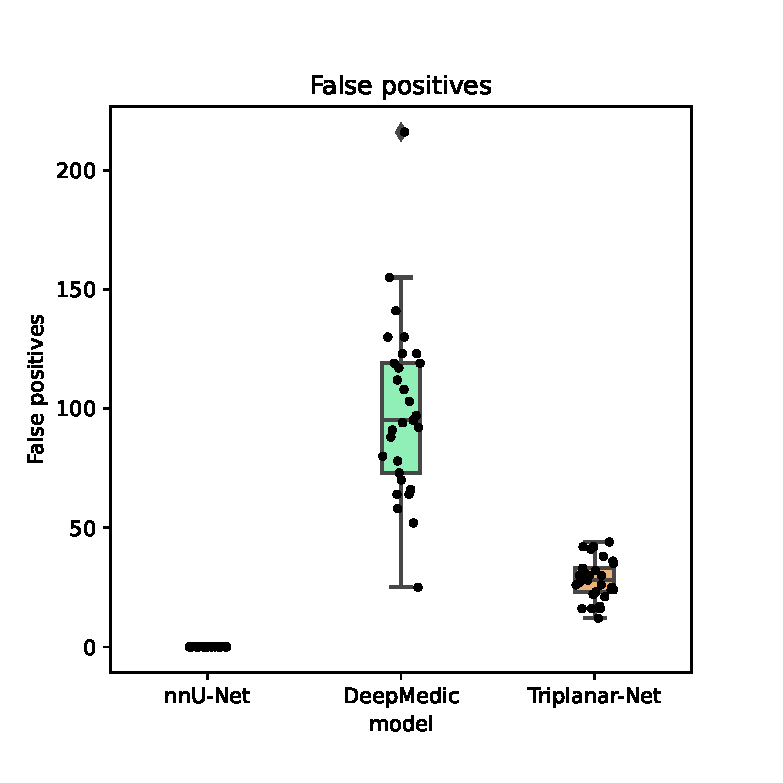
\includegraphics[width=\linewidth]{figures/FalsePositives.eps}
	\end{subfigure}
	\caption{Box plots of results shown for DSC, MHD, VS and false positives for each network architecture for the train dataset and bar plot shown for sensitivity of detections among network architectures (cont.).}
	\label{fig:results_cont}
\end{figure}
\begin{figure}
	\ContinuedFloat
	\centering
	\begin{subfigure}{.6\linewidth}
		\includegraphics[width=\linewidth]{figures/Sensitivity.eps}
	\end{subfigure}
	\caption{Box plots of results shown for DSC, MHD, VS and false positives for each network architecture for the train dataset and bar plot shown for sensitivity of detections among network architectures (cont.).}
	\label{fig:results_cont_cont}
\end{figure}

\section{Further evaluation}

\subsection{Inference}
Inference time and number of parameters of the three network architectures are shown in \ref{table:inference}; inference time is a very dependent result and to attempt to keep it as unbiased and normalized as possible, for all networks inference was done on an NVIDIA P100 GPU under equivalent conditions. The mean inference time is reported in seconds and calculated by taking an average of the time required for the forward pass of the network over all train data.

\begin{table}[h!tp]
	\centering
	\begin{tabular}{l r r }
		& parameters & mean inference time (s) \\
		\hline
		nnU-Net & 178297920 & 203 \\
		DeepMedic & \textbf{1178100} & 175 \\
		Triplanar-Net & 1478264 & \textbf{35} \\
	\end{tabular}
	\caption[Number of parameters and inference time.]{The number of parameters and mean inference time --for the forward pass -- of each network architecture across all train dataset cases.}
	\label{table:inference}
\end{table}

\subsection{Segmentation results of true UIAs}
For the three networks assessed, the segmentation performance for only true UIAs  was also evaluated, and the results are shown in Table \ref{table:metrics_pos}. This evaluation was only done on the train dataset.

\begin{table}[h]
	\centering
	\begin{tabular}{ l  r r r }
%		\multirow{3}{4em}{} & \multicolumn{3}{ c }{\textbf{Train}} \\
%		
		& \multirow{2}{2em}{DSC} & MHD & \multirow{2}{2em}{VS} \\
		& & (mm) & \\
		\hline
		%		3D U-Net & 0. & 0. & 0. & 0. & 0. & 0. \\
		nnU-Net & \textbf{0.91} & \textbf{0.47} & \textbf{0.88} \\
		DeepMedic & 0.25 & 7.99 & 0.37 \\
		Triplanar-Net & 0.23 & 10.07 & 0.27 \\
	\end{tabular}
	\caption[Segmentation results of true UIAs.]{The mean segmentation metrics of each network architecture evaluated on only true UIAs. Results in bold show the best value for that specific metric.}
	\label{table:metrics_pos}
\end{table}

\subsection{Performance on negative scans}
The average false positive count over all scans containing no true UIAs is shown in Table \ref{table:metrics_neg}, along with the false positive count for all scans. These results are only shown for the train dataset.

\begin{table}[h]
	\centering
	\begin{tabular}{ l  r r r }
		& All scans & Positive scans & Negative scans \\
		\hline
		nnU-Net & \textbf{0.00} & \textbf{0.00} & \textbf{0.00} \\
		DeepMedic & 99.41 & 97.04 & 110.80 \\
		Triplanar-Net & 28.17 & 28.00 & 29.00 \\
	\end{tabular}
	\caption[False positive count for all scans, positive scans and negative scans.]{The false positive count of each network architecture over all train cases for all scans, positive scans, and negative scans. Results in bold show the best value for that specific metric.}
	\label{table:metrics_neg}
\end{table}

\subsection{Sizes of UIAs}
In Figure \ref{fig:DSC_sizes.eps} diameter of the UIAs is split into four quartiles, and a bar plot of the DSC for the three evaluated networks is shown.

\img{DSC_sizes.eps}{0.6\linewidth}{Dice Score Coefficient of networks split into sizes of aneurysms.}{Box plot of the Dice Score Coefficients of each network architecture based on different UIA sizes, split into four quartiles.}

\subsection{Qualitative results}
Axial slices of three input TOF-MRA volumes overlayed with the segmented aneurysm are shown in Figure \ref{fig:qual_results} along with the ground truth labels.

\begin{figure}[htp]
	\centering
	\begin{subfigure}{\linewidth}
		\includegraphics[width=\linewidth]{figures/results_10049F.pdf}
	\end{subfigure}
	\begin{subfigure}{\linewidth}
		\includegraphics[width=\linewidth]{figures/results_10034.pdf}
	\end{subfigure}
	\begin{subfigure}{\linewidth}
		\includegraphics[width=\linewidth]{figures/results_10073F.pdf}
	\end{subfigure}
	\caption[Qualitative results of each network on three positive cases.]{The axial slices of three positive TOF-MRA volumes, showing the ground truth labels, the output segmentation of the nnU-Net architecture, the output segmentation of the DeepMedic architecture, and the output segmentation of the Triplanar-Net architecture in each row respectively.}
	\label{fig:qual_results}
\end{figure}
%\chapter{Conclusion}

%\minitoc\pagebreak


\section{I am a section}



\subsection{I am a subsection}

Citing: \cite{Sample2016}





% #################
% ### APPENDIX  ###
% #################

\chapter*{Acknowledgments}
%\addcontentsline{toc}{chapter}{Acknowledgments}
\thispagestyle{empty}

I would like to thank my advisor Supro for his technical support and his suggestions and ideas. The author of the ADAM challenge, Kimberley, was very responsive and helpful when first using the dataset and evaluating it on the test dataset. I would also like to thank Alessa, Luis and Saif for reading and going over my thesis and being as judgmental as they were without being cynical -- especially Alessa and Luis who also cooked food when I couldn't. I would also like to thank everyone in the IBBM research group for putting up with me using a lot of GPU resources for a while. Finally, I would like to thank my parents for always being there even when I went MIA for a few weeks at a time.

\cleardoublepage{}


%\part*{Appendix}
%
%\pagenumbering{Roman} % römische Ziffern für die Anhänge
%
%\begin{appendix}
%	\chapter{Appendix: Ablation study for network architecture design}
\label{appendix1}

Before arriving to the network architecture shown in Chapter \ref{chapter5} for Triplanar-Net, other network architectures were also designed with the same concept of attempting to employ the use of 2D MIPs to segment aneurysms in 3D TOF-MRA images. In particular, the BtrflyNet architecture, the BtrflyNet with an added third input arm -- Figure \ref{fig:triflynet.pdf}, and the BtrflyNet with a 3D decoder substituting the 2D decoder -- Figure \ref{fig:3dtriwingednet.pdf} were the networks tested. Small variations of these networks were also tested, such as removing the skip connection or varying the channels in each layer. All these architectures proved to not be able to even overfit well enough on data used to train the architecture, and thus the final iteration of Triplanar-Net was decided upon. The DSC of each network evaluated on full volumes of the cases used to train the network are shown in Table \ref{table:iterations}. Only the DSC is reported so as to only to show one necessary metric to evaluate the segmentation performance.

\img{triflynet.pdf}{\linewidth}{Design iteration 1. Proposed architecture for variation of BtrflyNet with an additional third input arm, taking inputs as axial, coronal and sagittal MIPs and obtaining axial, coronal and sagittal MIP labels.}{Design iteration 1.}

\img{3dtriwingednet.pdf}{\linewidth}{Design iteration 2. Proposed architecture for variation of design iteration 1 using a 2D to 3D reconstruction block and a 3D decoder.}{Design iteration 2.}

\begin{table}[htp]
	\centering
	
	\begin{tabular}{l | r}
		& DSC \\
		\hline
		Design iteration 1 & 0.14 \\
		Design iteration 1 (no skip) & 0.09 \\
		Design iteration 2 & 0.23 \\
		Design iteration 2 (with skip) & 0.37 \\
		Triplanar-Net & \textbf{0.62}
	\end{tabular}

	\caption[Evaluation on training data for architecture designs before Triplanar-Net.]{DSCs reported for full volumes of training data for design iterations and variations.}
	\label{table:iterations}
\end{table}

The issue with design iteration 1 was presumed to be that the complete loss of 3D context within this architecture manifests in a poor performing network; having to reconstruct the 3D binary output segmentation after obtaining the 2D MIP labels of each view could be changed to allow combining of the three labels in a less naive method. Therefore, it was opted to change to design iteration 2, in which a 3D decoder is used after reconstructing the 3D labels within the network using the 2D to 3D reconstruction block as mentioned in Chapter \ref{chapter5}. It was also interesting to see the addition and removal of skip connections in design iteration 2. Finally, to arrive at the chosen design for Triplanar-Net, the middle arm of design iteration 2 was removed as concatenating the intermediate features of the three input arms was hypothesized to not be a useful use of the processed features.

A further experiment was also carried out to use a 2-staged pipeline to segment aneurysms. The first stage being localizing the aneurysm, and the second stage involving the actual segmentation. The pipeline can be seen in Figure \ref{fig:full_pipeline.pdf}. The hope with using this 2-stage pipeline was to reduce false positives. In the end, although various architectures were attempted for the first stage, the specificity and sensitivity were too low to warrant using a 2-staged approach for the task. If a classifier network is unable to detect accurately enough whether a certain patch contains an aneurysm, than the chance of false negatives for the full pipeline would be drastically increased. This pipeline was experimented with various classifier networks and segmentation networks (with the iterations discussed), and the maximum sensitivity and specificity achieved (for the first stage) was 0.84 and 0.77 respectively.

\img{full_pipeline.pdf}{\linewidth}{Proposed 2-staged pipeline, incorporating classification of a specific input patch before performing segmentation. The hope is to reduce false positives, while not drastically increasing workload and amount of required resources.}{Proposed 2-staged pipeline for inference.}




		
%\end{appendix}

% Reset paragraph whitespace
\bigLineSpacing{OFF}

 \glsaddall{} % add all defined terms to glossary, even if not referenced in text
 \printglossaries{}
 
 \microtypesetup{protrusion=false}
 \listoffigures{}
 \listoftables{}
 \microtypesetup{protrusion=true}
 \printbibliography{}

\end{document}
